%  template.tex for Biometrics papers
%
%  This file provides a template for Biometrics authors.  Use this
%  template as the starting point for creating your manuscript document.
%  See the file biomsample.tex for an example of a full-blown manuscript.

%  ALWAYS USE THE referee OPTION WITH PAPERS SUBMITTED TO BIOMETRICS!!!
%  You can see what your paper would look like typeset by removing
%  the referee option.  Because the typeset version will be in two
%  columns, however, some of your equations may be too long. DO NOT
%  use the \longequation option discussed in the user guide!!!  This option
%  is reserved ONLY for equations that are impossible to split across 
%  multiple lines; e.g., a very wide matrix.  Instead, type your equations 
%  so that they stay in one column and are split across several lines, 
%  as are almost all equations in the journal.  Use a recent version of the
%  journal as a guide. 
%  
\documentclass[useAMS,referee, usegraphicx]{biom}
%\documentclass[useAMS, usegraphicx]{biom}
%
%  If your system does not have the AMS fonts version 2.0 installed, then
%  remove the useAMS option.
%
%  useAMS allows you to obtain upright Greek characters.
%  e.g. \umu, \upi etc.  See the section on "Upright Greek characters" in
%  this guide for further information.
%
%  If you are using AMS 2.0 fonts, bold math letters/symbols are available
%  at a larger range of sizes for NFSS release 1 and 2 (using \boldmath or
%  preferably \bmath).
% 
%  Other options are described in the user guide. Here are a few:
% 
%  -  If you use Patrick Daly's natbib  to cross-reference your 
%     bibliography entries, use the usenatbib option
%
%  -  If you use \includegraphics (graphicx package) for importing graphics
%     into your figures, use the usegraphicx option
% 
%  If you wish to typeset the paper in Times font (if you do not have the
%  PostScript Type 1 Computer Modern fonts you will need to do this to get
%  smoother fonts in a PDF file) then uncomment the next line
%  \usepackage{Times}
\usepackage{amsmath}
\usepackage{graphicx}
\usepackage{url}
\usepackage{bm}
\usepackage{amssymb}


%%%%% PLACE YOUR OWN MACROS HERE %%%%%

\def\bSig\mathbf{\Sigma}
\newcommand{\VS}{V\&S}
\newcommand{\tr}{\mbox{tr}}

%  The rotating package allows you to have tables displayed in landscape
%  mode.  The rotating package is NOT included in this distribution, but
%  can be obtained from the CTAN archive.  USE OF LANDSCAPE TABLES IS
%  STRONGLY DISCOURAGED -- create landscape tables only as a last resort if
%  you see no other way to display the information.  If you do do this,
%  then you need the following command.

%\usepackage[figuresright]{rotating}

%%%%%%%%%%%%%%%%%%%%%%%%%%%%%%%%%%%%%%%%%%%%%%%%%%%%%%%%%%%%%%%%%%%%%

%  Here, place your title and author information.  Note that in 
%  use of the \author command, you create your own footnotes.  Follow
%  the examples below in creating your author and affiliation information.
%  Also consult a recent issue of the journal for examples of formatting.

\title[Finite area smoothing with MDS]{Using multidimensional scaling, within-area distances and Duchon splines for finite area smoothing}


\author{David L. Miller$^{1*}$\email{dave@ninepointeightone.net}, Simon N. Wood$^{2}$\\
$^{1}$CREEM, University of St Andrews, The Observatory, Buchanan Gardens, St Andrews KY16 9LZ, Scotland\\
$^{2}$Dept of Mathematical Sciences, University of Bath, Claverton Down, Bath BA2 7AY, U.K.
}

\begin{document}

%  This will produce the submission and review information that appears
%  right after the reference section.  Of course, it will be unknown when
%  you submit your paper, so you can either leave this out or put in 
%  sample dates (these will have no effect on the fate of your paper in the
%  review process!)

%\date{{\it Received October} 2007. {\it Revised February} 2008.  {\it Accepted March} 2008.}

%  These options will count the number of pages and provide volume
%  and date information in the upper left hand corner of the top of the 
%  first page as in published papers.  The \pagerange command will only
%  work if you place the command \label{firstpage} near the beginning
%  of the document and \label{lastpage} at the end of the document, as we
%  have done in this template.

%  Again, putting a volume number and date is for your own amusement and
%  has no bearing on what actually happens to your paper!  

%\pagerange{\pageref{firstpage}--\pageref{lastpage}} 
%\volume{65}
%\pubyear{2008}
%\artmonth{December}

%  The \doi command is where the DOI for your paper would be placed should it
%  be published.  Again, if you make one up and stick it here, it means 
%  nothing!

%\doi{10.1111/j.1541-0420.2005.00454.x}

%  This label and the label ``lastpage'' are used by the \pagerange
%  command above to give the page range for the article.  You may have 
%  to process the document twice to get this to match up with what you 
%  expect.  When using the referee option, this will not count the pages
%  with tables and figures.  

\label{firstpage}

%  put the summary for your paper here

\begin{abstract}
This version: \today %Remove this before submitting!

YAKYAKYAK
\end{abstract}

%  Please place your key words in alphabetical order, separated
%  by semicolons, with the first letter of the first word capitalized,
%  and a period at the end of the list.
%

\begin{keywords}
Generalized additive model; splines; finite area smoothing.
\end{keywords}

%  As usual, the \maketitle command creates the title and author/affiliations
%  display 

\maketitle


%  If you are using the referee option, a new page, numbered page 1, will
%  start after the summary and keywords.  The page numbers thus count the
%  number of pages of your manuscript in the preferred submission style.
%  Remember, ``Normally, regular papers exceeding 25 pages and Reader Reaction 
%  papers exceeding 12 pages in (the preferred style) will be returned to 
%  the authors without review. The page limit includes acknowledgements, 
%  references, and appendices, but not tables and figures. The page count does 
%  not include the title page and abstract. A maximum of six (6) tables or 
%  figures combined is often required.''

%  You may now place the substance of your manuscript here.  Please use
%  the \section, \subsection, etc commands as described in the user guide.
%  Please use \label and \ref commands to cross-reference sections, equations,
%  tables, figures, etc.
%
%  Please DO NOT attempt to reformat the style of equation numbering!
%  For that matter, please do not attempt to redefine anything!
\section{Introduction \label{IN}}

A typical application of spline smoothing in ecological modelling consists of a response modelled as a function of its spatial coordinates. The estimated function can then be used to perform inference on the population, whether that be an abundance estimate, density map or as part of a larger model, taking into account nuisance spatial effects. Finite area smoothing concerns the situation in which the domain over which this smoothing takes place is bounded. 

Mathematically, we wish to model some response, $z_i$, as a smooth function of the spatial coordinates $(x_{1i}, x_{2i})$:
\begin{equation*}
z_i = f(x_{1i}, x_{2i}),
\end{equation*}
where $f$ is a sum of flexible basis functions. In order to avoid overfitting, a penalty based on integrating the squared derivatives of $f$ is calculated (see below). When normal errors are used the model is known as an additive model. The method described here can be used when the response has an exponential family distribution; the generalised addtive model case. Often smooths of spatial coordinates are used to explain autocorrelation in the data that may confound the actual relationships of interest. Here the focus is on simple smooths of spatial location, since these are the building blocks of the more complicated models.

When the geographical region has a \emph{complex boundary}, features from one part of the domain can unduly influence other parts. Considering the boundary as a polygon, a complex boundary is a non-convex polygon, in particular when the non-convexity is relatively extreme. Often this consists of having some peninsula-like feature(s) in the domain with notably different observation values on either side of the feature. Given that there is some scientific motivation as to why those parts of the domain should not affect each other, features such as peninsulae give rise to a phenomenon known as \emph{leakage}.

Leakage occurs when a smoother inappropriately links two pats of a domain (Wood, Bravington and Hedley, 2008). The phenomenon is problematic since it causes the fitted surface to be mis-estimated; this can then lead to incorrect inference (e.g. bias), which is clearly not desirable. Leakage can be seen in Figure \ref{leakage} where the high values in the upper half of the domain leak across the gap to the lower values below and vice versa.

% leakage example 
\begin{figure}
\centering
% trim order l b r t
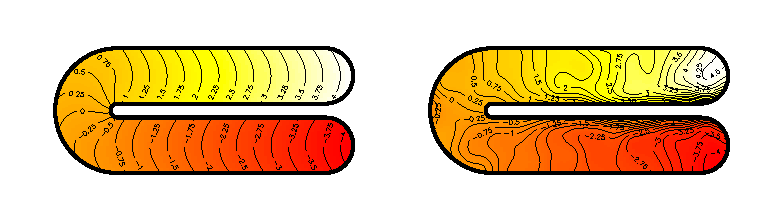
\includegraphics[width=\textwidth]{figs/ramsay-leak.ps}\\
\caption{An example of leakage on the modified Ramsay horseshoe (Wood et al, 2008). A thin plate regression spline was fit to data sampled from the function on the left, the model smooths across the gap in the middle of the domain (right).}
\label{leakage}
\end{figure}

The problem of leakage arises because of the way in which the smoother measures how near objects are to one another. Most smoothing techniques use the Euclidean metric to measure the distance between data. Clearly though, this approach is a flawed: biological populations do not conform to Euclidean geometry in their movement patterns and hence their observed positions will reflect this. Just as whales no not uniformly distribute themselves across sea and glacier, fish do not lay their eggs on land. Natural and man-made barriers carve up the landscape (and seascape), partitioning biological populations; spatial models should take this into account.

The distribution of the population may be smooth, just not necessarily over $\mathbb{R}^2$ (Wang and Ranalli, 2007). Modelling the structure of the domain correctly by embedding the extra information relating to the shape of the boundary (whether this be implicitly or explicitly) allows for more accurate inference.

The cause of leakage can be characterised in two ways: either the smooth does not respect the boundary of the domain, or the smooth does not take into account the geometry of the domain (in particular with regard to the distance between points within the domain). Previous work in this area has been to combat leakage along these two lines. Work of Ramsay (2002) and Wood et al. (2008) both use a partial differential equation (PDE) boundary condition approach to try to prevent leakage, where as Wang and Ranalli (2007) and Eilers (2006) modify the way that inter-point distances are measured in order to avoid smoothing across boundaries. These four main works are summarised in the next section.

This article addresses the problem of leakage in the additive model case. The methods elaborated on here may then be extended to the generalized additive case, since they merely represent a more convenient basis setup for such models. The article proceeds as follows: section \ref{previous-approaches} highlights previous approaches to the problem of leakage, section \ref{proposed-model} illustrates the proposed model, section \ref{examples} gives examples of the method at work (along with comparisons to the current best methodology). Finally, section \ref{conclusion} compares the proposed method with similar approaches in the kriging literature and discusses further work.

\section{Previous approaches to the problem of leakage}
\label{previous-approaches}

FELSPLINE (2002 and 2011)... LINK between... soap Marra et al!

Wang and Ranalli .. link to Eilers

Lindesay and Carl's paper?


Say something about investigation of SC methods, REF thesis

\section{Model definition}
\label{proposed-model}

Multidimensional scaling (MDS) or, as it is often referred to, principle coordinates (PCO) (Gower, 1966) is a method commonly used in multivariate analysis. MDS takes a (symmetric) matrix of distances between the observations projects the data in such a way that Euclidean inter-point distances in the projected space are approximately the same as the distances which make up the entries of the matrix (Chatfield and Collins, 1980, Chapter TKTKTK). If the matrix of distances is of rank $n$ then the projection can be in $n-1$ or less dimensions; a projection into 2 dimensions is a typical choice, since it is easily visualised. When MDS is performed on some categorised set of dissimilarities (as is often the case in social science and psychology) it is referred to as non-metric MDS, where as on a continuous scale it is known as metric MDS. Discussion here will focus on metric MDS.

Multidimensional scaling provides a way to transform a domain. Given the set of distances between points in a domain, we can project those points into a configuration such that the distances between those points are approximately preserved. Now, if the Euclidean metric were to be used to calculate the distances between the points then the result from the projection would be identical (up to rotation and translation) to the starting point configuration (provided that the projection had the same number of dimensions as the original data). However, if it were possible to use a metric that took into account the distance within the boundary (a \textit{within-area distance}) then the Euclidean distances between points in the resulting configuration would be (approximately) the same as the within-area distances. This would lead to distances used by the basis functions of the smoother to be approximately the within-area distances.

Mathematically, MDS takes a matrix of squared distances ($\mathbf{D}$, say), and eigen-decomposes it: $\mathbf{D}=\mathbf{U}\mathbf{\Lambda}\mathbf{U}^\text{T}$, where $\mathbf{U}$ is a matrix with orthogonal columns which are the eigenvectors and $\mathbf{\Lambda}$ is  a diagonal matrix of eigenvalues in decreasing absolute value order along the diagonal. Truncating $\mathbf{U}\mathbf{\Lambda}^{1/2}$ to say, the first $k$ columns gives the projected space. [[TKTKTK better]]

Biological populations respect the intrinsic structure of these domains and in general do not respect Euclidean geometry in their movement patterns (for example, they move around obstacles, avoid predators and track prey). When within-area distances are meaningful, it makes sense to include the structure of the domain in the model, rather than somewhat arbitrarily choose Euclidean geometry and discard this extra information. However, as literature on smoothing is firmly based in a Euclidean context, it would be preferable to perform the smoothing in Euclidean space. In this case the approximation to Euclidean space afforded by an MDS projection of the within-area distances offers a bridge between these two requirements.

By using within-area distances, we encapsulate information about the boundary into the model in an implicit way (in contrast to Wood et al, 2008 and Ramsay, 2002) so that the boundary enters the model via the points rather than as a special structure.

The procedure to fit the model is as follows: given the sample locations $\mathbf{x}_i = (x_{1i}, x_{2i})$  of the $i^\text{th}$ point with response $z_i$ (in general $\mathbf{x}_i$ could be $k$-vector, although 2-vectors of geographical coordinates are used throughout this chapter). Then:
\begin{enumerate}
\item Obtain the MDS configuration for the domain using some representative set of points over the area in question. The only use of the MDS locations obtained in this step is to find the initial MDS configuration; they are discarded afterward. Representative points could be a sparse grid over the domain or a subset of $\{\mathbf{x}_i : i=1\dots n\}$. More detail and justification is provided in Appendix A.
\item Using the MDS configuration obtained above along with Gower's interpolation (Gower, 1968, see Appendix A) to obtain the location of the sample in the MDS configuration: $\{\mathbf{x}_i^*, z_i : i=1\dots n\}$.
\item Smooth $\{\mathbf{x}_i^*, z_i : i=1\dots n\}$ using a penalised regression spline.
\end{enumerate}
To predict at a location $\mathbf{x_j}$ in the original domain, use Gower's interpolation to obtain the point's location in the MDS space: $\mathbf{x}_j^*$. Predict $\hat{f}(\mathbf{x}_j)$.

Here, finding an MDS configuration of a set of points consists of: $i$) calculating the within-area distances between the points, $ii$) forming the distance matrix and, $iii$) actually performing the MDS projection; the details of each step are covered in the following sections.

Preliminary experiments were carried out using a 2-dimensional projection of the distance matrix. Figure \ref{wt2-plot} shows that when a domain with peninsulae is projected using MDS with within-area distances, the resulting point configuration appears squashed. This can actually cause the ordering of the points to be lost, making the task of the smoother impossible. Further investigation shows that in higher dimensions the projection maintains the ordering of the points while avoiding leakage.

\subsection{Smoothing with Duchon splines}

In the preceding investigations, the thin plate regression splines of Wood (2003) were used. This formulation has many nice properties: they are eigen-based and do not require knot selection, they are isotropic, they are relatively fast to fit and they are implemented in software (the \texttt{mgcv} package for \textsf{R}). However, high-dimensional smoothing using thin plate regression splines can be rather tricky, this is because the size of the nullspace (the functions which make up the spline that are not penalised) is a function of the smoothing dimension. This leads to a model containing a large set of unpenalised functions which can lead to overfitting.

When originally proposing thin plate splines in his seminal 1977 paper, Duchon actually describes a much more general set of interpolation methods; thin plate splines are just a particular example of these. This more general version of the thin plate spline (henceforth referred to as \textit{Duchon splines}) can be used for high dimensional smoothing whilst avoiding a large and complex penalty nullspace. Duchon splines have been largely neglected in statistical smoothing literature with the exception of Girosi, Jones and Poggio (1995) which discusses the connections between neural networks and GAMs. Hastie, Tibshirani and Friedman (2001, p. 168) discuss Girosi's work briefly.

The here aim is to show how the penalty works and that the main differences between it and the thin plate spline penalty; a full technical exposition (from a mathematical rather than statistical point of view) is given in Duchon (1977). Starting from the definition of the thin plate spline penalty and shows how one can motivate the more general Duchon spline penalty. 

The thin plate spline penalty (e.g. Wood, 2003) in $d$ dimensions with derivative order $m$ is :
\begin{equation}
J_{m,d} = \int \ldots \int_{\mathbb{R}^d} \sum_{\nu_1 + \dots + \nu_d=m} \frac{m!}{\nu_1! \dots \nu_d!} \left( \frac{\partial^m f \left (x_1,\dots,x_d \right )}{\partial x_1^{\nu_1} \ldots  \partial x_d^{\nu_d}} \right)^2 \text{d} x_1 \ldots  \text{d} x_d,
\label{tprs-pen}
\end{equation}
where the summation index generates all of the possible combinations of derivative orders such than their sum is still $m$ (thereby finding all the correct cross-terms for the derivatives). In order to ensure that $f$ remains continuous, $2m>d$.

It can then be shown that the minimiser of (\ref{tprs-pen}) is the thin plate spline basis:
\begin{equation}
f(\mathbf{x}) = \sum_{i=1}^n \delta_i \eta_{md}(\mathbf{x}-\mathbf{x_i}) + \sum_{j=1}^M \alpha_j \phi_j(\mathbf{x}),
\label{tprs-basis}
\end{equation}
where the first summation is a set of radial basis functions ($i$ indexing the $n$ data) and the second summation are a set of linearly independent polynomials of degree less than $m$. The terms in the second summation are unpenalized since their $m^\text{th}$ derivatives are zero. There are $M$ of these polynomials lying in the nullspace of the penalty, where $M$ is given by:
\begin{equation}
M=\begin{pmatrix} m+d-1 \\ d  \end{pmatrix}.
\label{gds-bigm}
\end{equation}
In the cases presented so far, $d$ (the MDS projection dimension) is known and $m$ is dictated by $d$, since $2m>d$. $M$ therefore increases very quickly with the number of dimensions; this is shown by the blue line in figure \ref{nullspace-dim}. As more basis functions are included in the nullspace, the more wiggly the functions are. A large number of increasing complex, global functions which are unpenalized pose a serious threat to the fitting of parsimonious models.

\begin{figure}
\centering
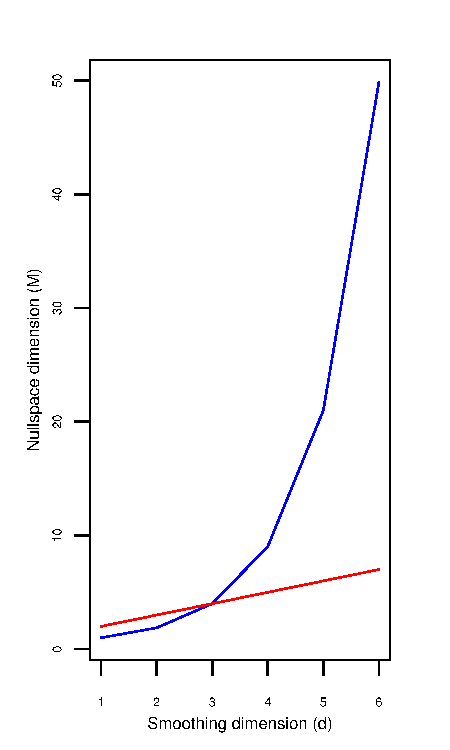
\includegraphics[width=3in]{figs/nullspace-dim.ps} \\
\caption{Relationship between smoothing dimension ($d$) and the nullspace dimension ($M$) when $m$ (the derivative penalty order) is set to 2 for thin plate regression splines (blue) and Duchon splines (red). Note that as the nullspace dimension increases, the complexity of those functions in the nullspace increases too. For the thin plate splines a combination of the continuity condition that $2m>d$ and the form of $M$ (see (\ref{gds-bigm})) makes the size of the nullspace increase very quickly with smoothing dimension. BLACK AND WHITE!!!}
\label{nullspace-dim}
% generated by thesis/mds/figs/nullspace-dim.R
\end{figure}

Starting from (\ref{tprs-pen}), the first step toward the more general Duchon penalty is to consider taking the Fourier transform of the derivatives before squaring and integrating them. Taking the Fourier transform of the derivatives in the penalty allows us to think of how the penalty is calculated in a different way. Rather than integrating the field of derivatives over space, the penalty is calculated from measuring the intensity of the different frequencies of the derivatives over the whole domain. Intuitively, the low frequency components of the derivatives of $f$ are likely performing a similar task to those functions in the nullspace of the penalty, where as the more complicated, high frequency components are more complicated parts of the function, likely to be the parts of $f$ that attempt to interpolate the data.

Taking the Fourier transform of the derivative terms in (\ref{tprs-pen}) yields the following penalty:
\begin{equation}
J_{m,d} = \int \ldots \int_{\mathbb{R}^d} \sum_{\nu_1 + \dots + \nu_d=m} \frac{m!}{\nu_1! \dots \nu_d!} \left ( \mathfrak{F} \frac{\partial^m f}{\partial x_1^{\nu_1} \ldots  \partial x_d^{\nu_d}} \left (  \boldsymbol{\tau}\right ) \right )^2 \text{d} \boldsymbol{\tau}.
\label{tprs-pen-ft}
\end{equation}
The penalties (\ref{tprs-pen}) and (\ref{tprs-pen-ft}) are in fact equivalent by Plancherel's theorem (e.g. Vretblad, 2003, p. 180) in the sense that they evaluate to the same numerical value.

Exploiting this frequency interpretation, it then follows to introduce a weighting into the penalty: 
\begin{equation}
\int \ldots \int_{\mathbb{R}^d} w(\boldsymbol{\tau}) \sum_{\nu_1 + \dots + \nu_d=m} \frac{m!}{\nu_1! \dots \nu_d!} \left ( \mathfrak{F} \frac{\partial^m f}{\partial x_1^{\nu_1} \ldots  \partial x_d^{\nu_d}} \left (\boldsymbol{\tau} \right ) \right )^2 \text{d} \boldsymbol{\tau},
\label{duchon-penalty-general}
\end{equation}
the function $w$ can then be used to pick out particularly high frequencies and penalize those more than the lower frequency ones. Setting $w(\boldsymbol{\tau})=1, \forall \boldsymbol{\tau}$ recovers (\ref{tprs-pen}).

Duchon suggests the use of $w(\boldsymbol{\tau})= \lvert \boldsymbol{\tau} \rvert^{2s}$. This will still give a minimiser of broadly the same form as the thin plate spline functions in (\ref{tprs-basis}) but $M$ will change. First writing down this penalty:
\begin{equation}
\breve{J}_{m,d} = \int \ldots \int_{\mathbb{R}^d} \lvert \boldsymbol{\tau} \rvert^{2s} \sum_{\nu_1 + \dots + \nu_d=m} \frac{m!}{\nu_1! \dots \nu_d!}\left ( \mathfrak{F} \frac{\partial^m f}{\partial x_1^{\nu_1} \ldots  \partial x_d^{\nu_d}} \left (\boldsymbol{\tau} \right ) \right )^2 \text{d} \boldsymbol{\tau}.
\label{duchon-penalty}
\end{equation}
The less complex (more smooth) frequency components of the basis functions are penalised less. This allows some of the frequencies of  the radial basis functions to do the job of the $M$ linearly independent polynomials which were not included due to reduced nullspace size. The penalty allows the use of a reduced nullspace (in both size and complexity terms) while not sacrificing the continuity of $f$. 

Again, (\ref{tprs-pen}) can be recovered from this penalty (by setting $s=0$). When $s>0$ higher frequencies are penalised more than lower ones. In order to obtain smooth functions it is required that $m+s>d/2$ (this replaces the condition $2m>d$). Using a value of $s>0$ allows for high dimensional smoothing while still using lower-order penalties without yielding discontinuous functions. One can therefore think of $s$ as a kind of ``fudge factor'' that allows the conditions on $m$ and $d$ to be relaxed. Given some fixed combination of $m$ and $d$, an $s$ can be found by simply calculating $s>d/2-m$. For the examples below, the smallest $s$ is used with $m=2$, so:
\begin{equation}
s=d/2-1.
\label{duchon-s-eqn2}
\end{equation}

The red line in figure \ref{nullspace-dim} gives the number of functions that lie in the nullspace of penalty (\ref{duchon-penalty}), i.e. the result of using (\ref{duchon-s-eqn2}) with (\ref{gds-bigm}). For plotting $m=2$ so the derivative order is constant as the dimensionality increases, leading to a linear increase in nullspace size with the smoothing dimension.

Note that the eigen-decomposition technique for avoiding knot selection for thin plate splines from Wood (2003) can be used with Duchon splines and is used in all of the examples in this article.

\subsection{Selecting the MDS projection dimension}

Given that the use of Duchon splines allows for reliable high dimensional smoothing, there is only one remaining issue to address. How many dimensions should the points be projected into. Setting the number of dimensions to project into to be the same for every domain surely seems like a recipe for disaster since even if this number of dimensions was set high enough to be acceptable for all domains, there would be some, simpler domains for which this would be far too high, wasting computational time. One option would be to select the number of dimensions according to the proportion of variation in the distances explained by the projection, however this too is somewhat subjective.

Rather than using either of the above methods, the GCV score was used. This exploits the fact that the time-consuming part of model fitting is the calculation of the within-area distances; fitting the model is cheap. So, fitting a series of models for projections from 2-dimensional upwards does not take significantly longer than fitting a single model, once the within-area distances have been calculated. Once a set of GCV scores have been calculated, the dimension which gives the lowest GCV is used as the final model. There is no particular reason to think that the score should be unimodal in the number of dimensions, so a full search is performed. In practise an upper bound of the number of dimensions that explained 95\% of the variation in the distances was used in the analyses shown below.

[[figure of score/dimension??]]

[[ML not so good, REML can't be used]]

\section{Examples}
\label{examples}

To illustrate the utility of the model two simulation studies are shown, followed by some examples on real data. In each case the method[[!!!]] was compared with thin plate splines (which do not account for the boundary) and the soap film smoother (which does).

\subsection{Ramsay's horseshoe}

The horseshoe shape shown in Figure \ref{leakage} is an obvious benchmark for techniques that wish to combat leakage. Although perhaps unrealistic (and bordering on pathological), any new methods that works well on the horseshoe should have a good chance of working well in other situations. A simulation experiment was run in which 200 replicates were generated at each combination of three error levels (standard normal noise multiplied by $(0.1,1,10)$) and three sample sizes (100, 300, 600). Other aspects of the setup were exactly as in Wood et al. (2008), a thin plate regression spline, (Wood, 2003), with basis size 100 and a soap film smoother with 32 interior knots  and a 40 knot cyclic  spline was used to estimate the boundary. For the mdsds model, the basis size was set to 100 and a 20 by 20 initial grid was used for the MDS projetion (see Appendix A), MDS projection dimensions was selected by GCV in the range of 2 and the number of dimensions that explained 95\% of the variation in the distance matrix of the initial grid. Smoothing parameters were selected by GCV. For each realisation the mean squared error (MSE) was calculated between the true function and a prediction grid of 720 points.

\begin{figure}
\centering
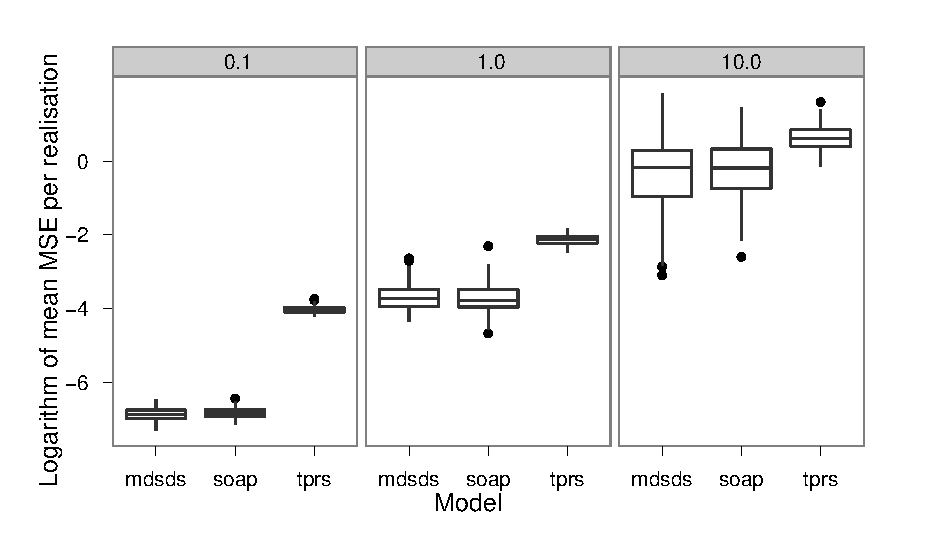
\includegraphics[width=\textwidth]{examples/ramsay/ramsay-result.eps} \\ 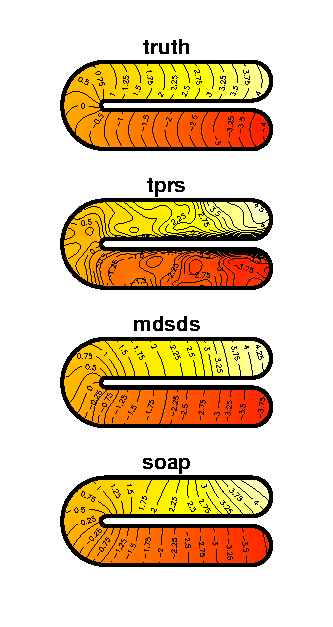
\includegraphics[width=\textwidth]{examples/ramsay/ramsay-real.eps}
% TKTKTK uncomment the above!
\caption{Top: boxplots of per-realisation $\log$ mean squared error at the three noise levels (rows) and sample sizes (columns). Using a paired Wilcoxon signed two-sample test, in every case the thin plate regression spline model (``tprs'') was found to be significantly worse than the soap film smoother (``soap'') at the 0.05 level. The new approach (``mdsds'') was only significantly different in two situations: sample size 300, noise level 10 (where it was worse, i.e. higher MSE) and sample size 600 with noise level 0.1 (where it was better, i.e. lower MSE). Bottom: typical predictions from the three models when the noise level was 1 and the sample size was 300. The prediciton grid used were was much finer than the one used for the MSE calculation above.}
\label{ramsay-results}
% generated by examples/ramsay/ramsay-plot.R
\end{figure}

As can be seen in Figure \ref{ramsay-results}, the thin plate regression spline has rather poor performance in MSE terms while MDSDS performs similarly well to soap. The median number of dimensions selected for the MDS projection using GCV was 3 (max. 14, min. 2). Looking more qualitatively at the bottom part of Figure \ref{ramsay-results}, the image plots do not show any evidence of leakage.


\subsection{Peninsulae}

The results from the modified Ramsay horseshoe are encouraging. However, as mentioned above, the problem is rather pathological and not particularly realistic. To further explore the performance of mdsds a more realistic domain (which attempts to mimic a coastline) was used. The domain is shown in Figure \ref{wt2-plot}.

Again, simulations were run at a series of noise levels 0.35,0.9 and1.55 equating to signal-to-noise ratios of 0.50, 0.75 and 0.95). The soap film smoother used 109 internal knots and the cyclic boundary smooth used 60. The mdsds models used an initial grid of 126 by 126 points, the basis size was 140. The thin plate regression spline basis was also of size 140.

\begin{figure}
\centering
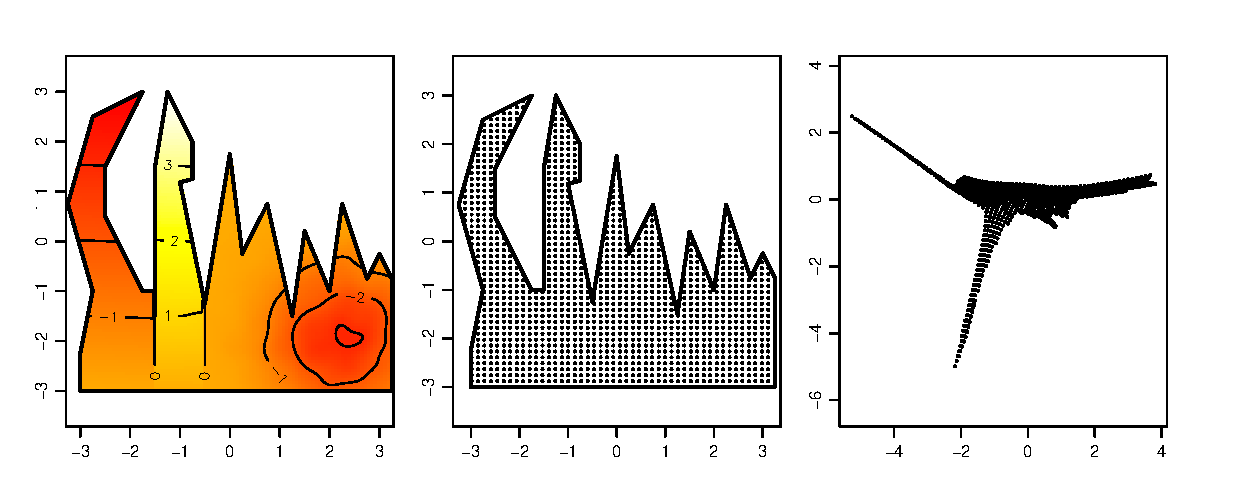
\includegraphics[width=\textwidth]{examples/wt2/wt2-plot.eps} \\
\caption{}
\label{wt2-plot}
% generated by examples/wt2/wt2-plot.R
\end{figure}


BOXPLOTS


\subsection{Aral sea}

%\subsection{Italy?}

\section{Discussion}
\label{conclusion}





\subsection{Comparison to kriging approaches}

%Kriging is focused on the explicit modelling of the correlations between points in space as a function of the distance between them via the estimation of the semivariogram. It is therefore logical that in, say, a river system the distances between points are calculated along the river's course rather than the Euclidean distance. 
%
%For the semivariogram to be a valid covariance function, it must be positive definite or conditionally negative definite (see \cite[p. 47]{diggle} for more information). However when non-Euclidean distances are used the semivariogram may no-longer fulfil either of these conditions (\cite{curriero}). The work of \citeb{mdskrig} attempts to solve this problem by using multidimensional scaling to project water distances into Euclidean space. Distances are not found exactly, a series of approximations are used rather than directly calculating the distances between the data. First the domain in question is triangulated, then the ``river distance'' between all of the nodes in the triangulation are calculated via Dijkstra's algorithm. The river distances are then projected using MDS. Finally, the data locations are mapped into the MDS space by interpolating between the grid points from the triangulation in MDS space.  The Euclidean distances in MDS space are then used in the estimation of the semivariogram. There are a number of issues with this approach. 
%
%Most prominently, the authors only consider ordinary kriging (where the mean process is treated as constant). In this case spatial variation only enters the model through the semivariogram.The effect of using the MDS projected points for a spatially varying mean process (in addition to the estimation of the semivariogram) has not been investigated. Prevailing opinion is that only polynomial trends should be used for the mean process (\cite[p. 57]{diggle}), how such an approach would perform in higher dimensions is not clear.
%
%Although the approximations used undoubtedly decrease the computational time, the validity of the approximations is not tested, especially on the fitting of the semivariogram (\cite{crabkrig}). The discretisation of the domain necessary to compute the graph distance via Dijsktra's algorithm has similar pitfalls to \citeb{wangranalli}. \citeb{crabkrig} suggest using the proportion of variation explained or the Bayesian criterion of \citeb{ohraftery} as possible metrics to perform projection dimension selection but do not full address the issue, resorting to 2-dimensional projections. Neither of the proposed selection methods take into account the effect that the dimension of the MDS projection has on the overall model (as discussed in \secref{gds-dimselect}).  \citeb{boisvert} suggest that to best approximate the distances, an $n-1$ dimensional projection of the distance matrix (if there are $n$ data, or triangulation nodes) be used (which is of course true) however they go on to point out that the use of such a high-dimensional projection could lead to numerical problems. Interpolating to find the distances in higher dimensions may also have it's own issues and so the approximations may run into further problems. In all of these works the MDS projection is being used to approximate the within-area distances by a set of distances obeying the rules of a Euclidean metric (the criterion given by \cite{curriero} to ensure valid semivariograms). Unlike in the material presented here, the MDS point configuration itself is not being used except to obtain a Euclidean approximation to the distances matrix so that the semivariogram can be estimated.
%
%In general kriging methods suffer from having developed as an \textit{ad hoc} set of tools used in the mining industry (\cite[preface]{diggle}). Although much work has been done to improve the mathematical basis of kriging, models are not as flexible as GAMs, in particular the incorporation of other covariates, temporal effects and random effects is not straight forward as it is for additive and generalized additive models (in both theory and practise).




\section*{Acknowledgements}



% Appendices
\section*{Appendix A - Using starting grids for stable MDS insertion}

Gower's interpolation!


\section*{Appendix B - Algorithm for the calculation of within-area distances}

remember to include the speed-up stuff






\begin{thebibliography}{99}

\bibitem{} Chatfield, C. and Collins, A.J. (1980). \textit{Introduction to multivariate analysis}. CRC Press.

\bibitem{} Girosi, F., Jones, M. and Poggio, T. (1995). Regularization theory and neural networks architectures. \textit{Neural computation}, \textbf{7}, 219-269.

\bibitem{} Gower, J.C. (1966). Some distance properties of latent root and vector methods used in multivariate analysis. \textit{Biometrika}, \textbf{53}(3 and 4), 325--338.

\bibitem{} Gower, J.C. (1968). Adding a point to vector diagrams in multivariate analysis. \textit{Biometrika}, \textbf{55}(3), 582--585.

\bibitem{} Gu, C. and Wahba, G. (1993). Smoothing Spline ANOVA with Component-Wise Bayesian Confidence Intervals. \textit{Journal of Computational and Graphical Statistics}, 2, 97--117.

\bibitem{} Hastie, T. and Tibshirani, R. (1990). \textit{Generalized Additive Models}. Chapman \& Hall.

\bibitem{} Hastie, T., Tibshirani, R. and Friedman, J. (2001). \textit{Elements of Statistical Learning}. Springer.

\bibitem{} Marra, G. and Radice, R. (2010). Penalised regression splines: theory and application to medical research. \textit{Statistical Methods in Medical Research}, 19, 107--125.

\bibitem{} Miller, D.L. (2011) \textit{On smooth models for complex domains and distances}. PhD thesis, University of Bath.

\bibitem{} Ramsay, T. (2002). Spline smoothing over difficult regions. \textit{Journal of the Royal Statistical Society Series B}, 64, 307--19.

\bibitem{} Ruppert, D., Wand, M.P. and Carroll, R.J. (2003). \textit{Semiparametric Regression}. Cambridge University Press.

\bibitem{} Vretblad, A. (2003). \textit{Fourier Analysis and Its Applications}. Springer.

\bibitem{} Wood, S.N. (2003). Thin plate regression splines. \textit{Journal of the Royal Statistical Society: Series B}, \textbf{65}(1), 95--114.

\bibitem{} Wood, S.N. (2006). \textit{Generalized Additive Models: An Introduction with R}. Chapman \& Hall.

\bibitem{} Wood, S.N. (2011). Fast stable restricted maximum likelihood and marginal likelihood estimation of semiparametric generalized linear models. \textit{Journal of the Royal Statistical Society Series B}, 73, 3--36.

\bibitem{} Wood, S.N., Bravington, M.V. and Hedley, S.L. (2008). Soap film smoothing. \textit{Journal of the Royal Statistical Society Series B}, 70, 931--55.

\end{thebibliography}


\label{lastpage}

\end{document}

